\subsection{\href{\linkpalrobotics}{PAL Robotics}}
   \hypertarget{subsec:pal_robotics}
   I begin working on the firmware for the fresh new roboot \href{https://pal-robotics.com/robots/kangaroo/}{\emph{Kangaroo}}. I study the hardware platform, main SoC capabilities and then a master plan was designed.
     \begin{figure}
      \begin{center}
         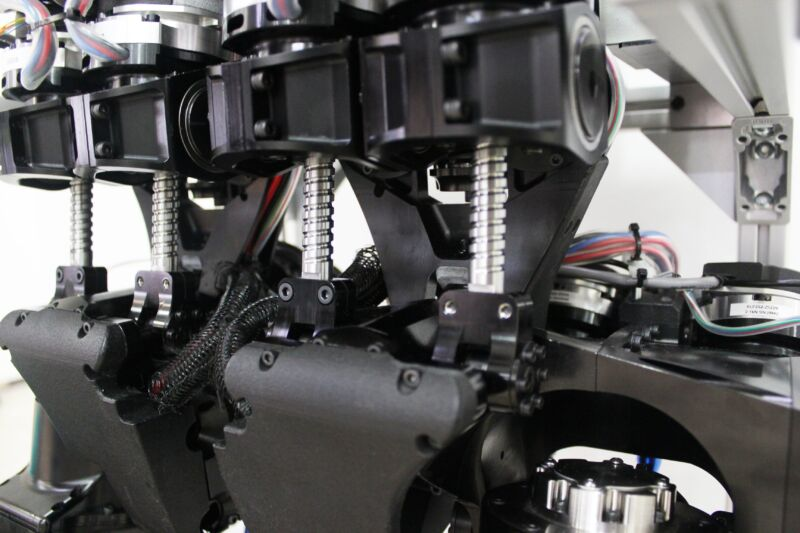
\includegraphics[width=0.3\textwidth]{pal_robotics1.jpg}
         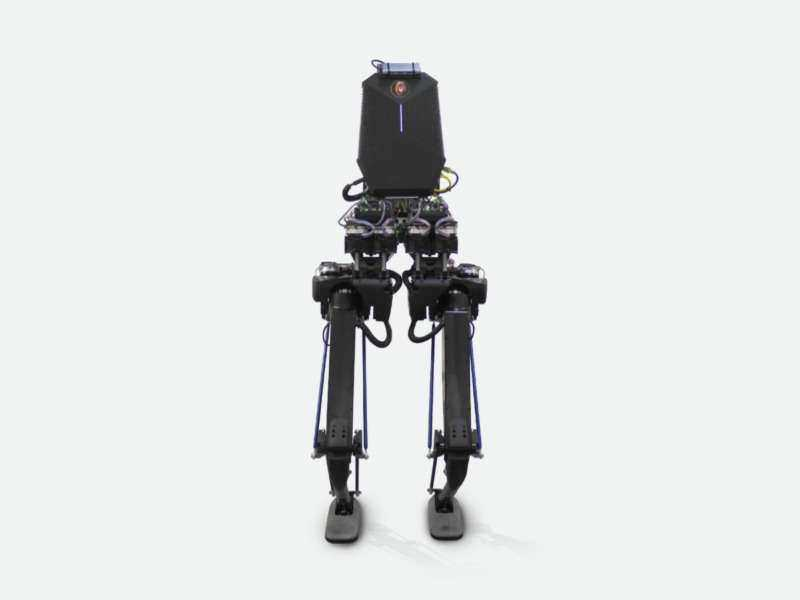
\includegraphics[width=0.3\textwidth]{pal_robotics2.jpg}
         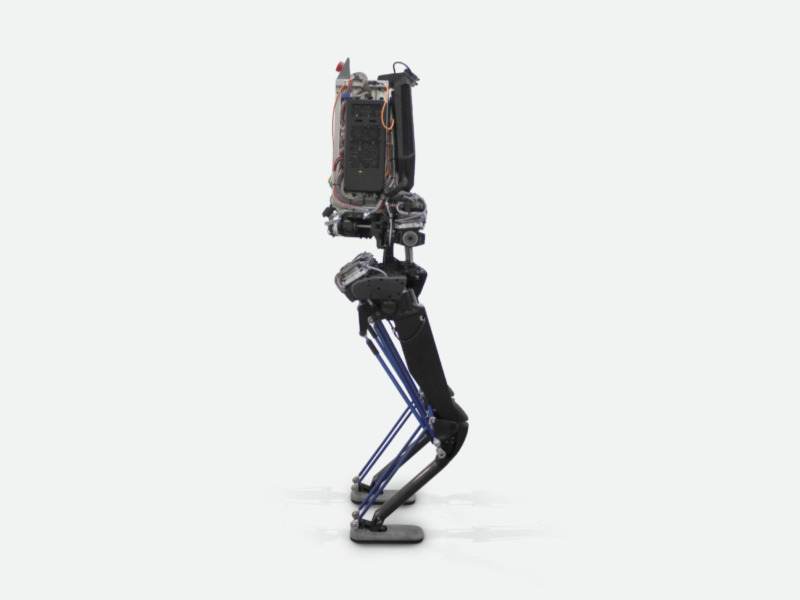
\includegraphics[width=0.3\textwidth]{pal_robotics3.jpg}
      \end{center}
        \caption{Fresh new robot from PAL Robotics \href{https://pal-robotics.com/robots/kangaroo/}{\emph{Kangaroo}}. It has a new mechanics and extremely powerful electronics. I work on the motors control loop, bootloaders and software in general running on it.}
      \label{fig:pal_robotics}
   \end{figure}

%---------------------------------------------------
\ifdefined\portfolioFull
   During my job at \href{\linkpalrobotics}{PAL Robotics} I mainly work as a bootloader and control loops firmware design and developer engineer.
   The actual core is in fact a 5x core: 1xARM Cortex + 2x C2000 architecture + 2 small but fast cores with custom RISC architecture.

   I've actually work on topics like:

         \cvlistitem{Design the main architecture of the bootloader taking in account the restricted resources}
         \cvlistitem{Design the IPC for inter processors communication}
         \cvlistitem{Implement a baremetal framework with full featured CLI to interact with the bootloader}
         \cvlistitem{Implement a realtime time and frequency visualizer over EtherCAT and UART using matplotlib + numpy}
         \cvlistitem{Implement a persistent telemetry over EtherCAT and UART with custom Json lib converter to a bootloader <-> CLI <-> python -> influxDB <- Grafana}
         \cvlistitem{"Three cores one code" pattern to reuse the same files for each core with minor changes related to hardware, architecture and memory layout multiplexed using makefiles and \#ifdef's}
         \cvlistitem{Implement a hex files receiver on C2000 core and a hex file sender in python both from scratch.}
         \cvlistitem{Using CLI + file sender + hex file parser + flash\_burn/ram API, the firmware update for any/all cores is just a text file script, and this is one of the more powerful feature achieved until now.}
         \cvlistitem{I began the implementation of a CI/CD and runners over PAL's gitlab server. They already have being using that for software, but not for firmware neither hardware.}
         \cvlistitem{Help my partners with some ideas on how to improve actual servo drive loop and firmware questions in general}
         \cvlistitem{Work with CLI git, push on gitlab servers, Agile environment with weekly reports and meetings.}

        \begin{figure}
         \begin{center}
            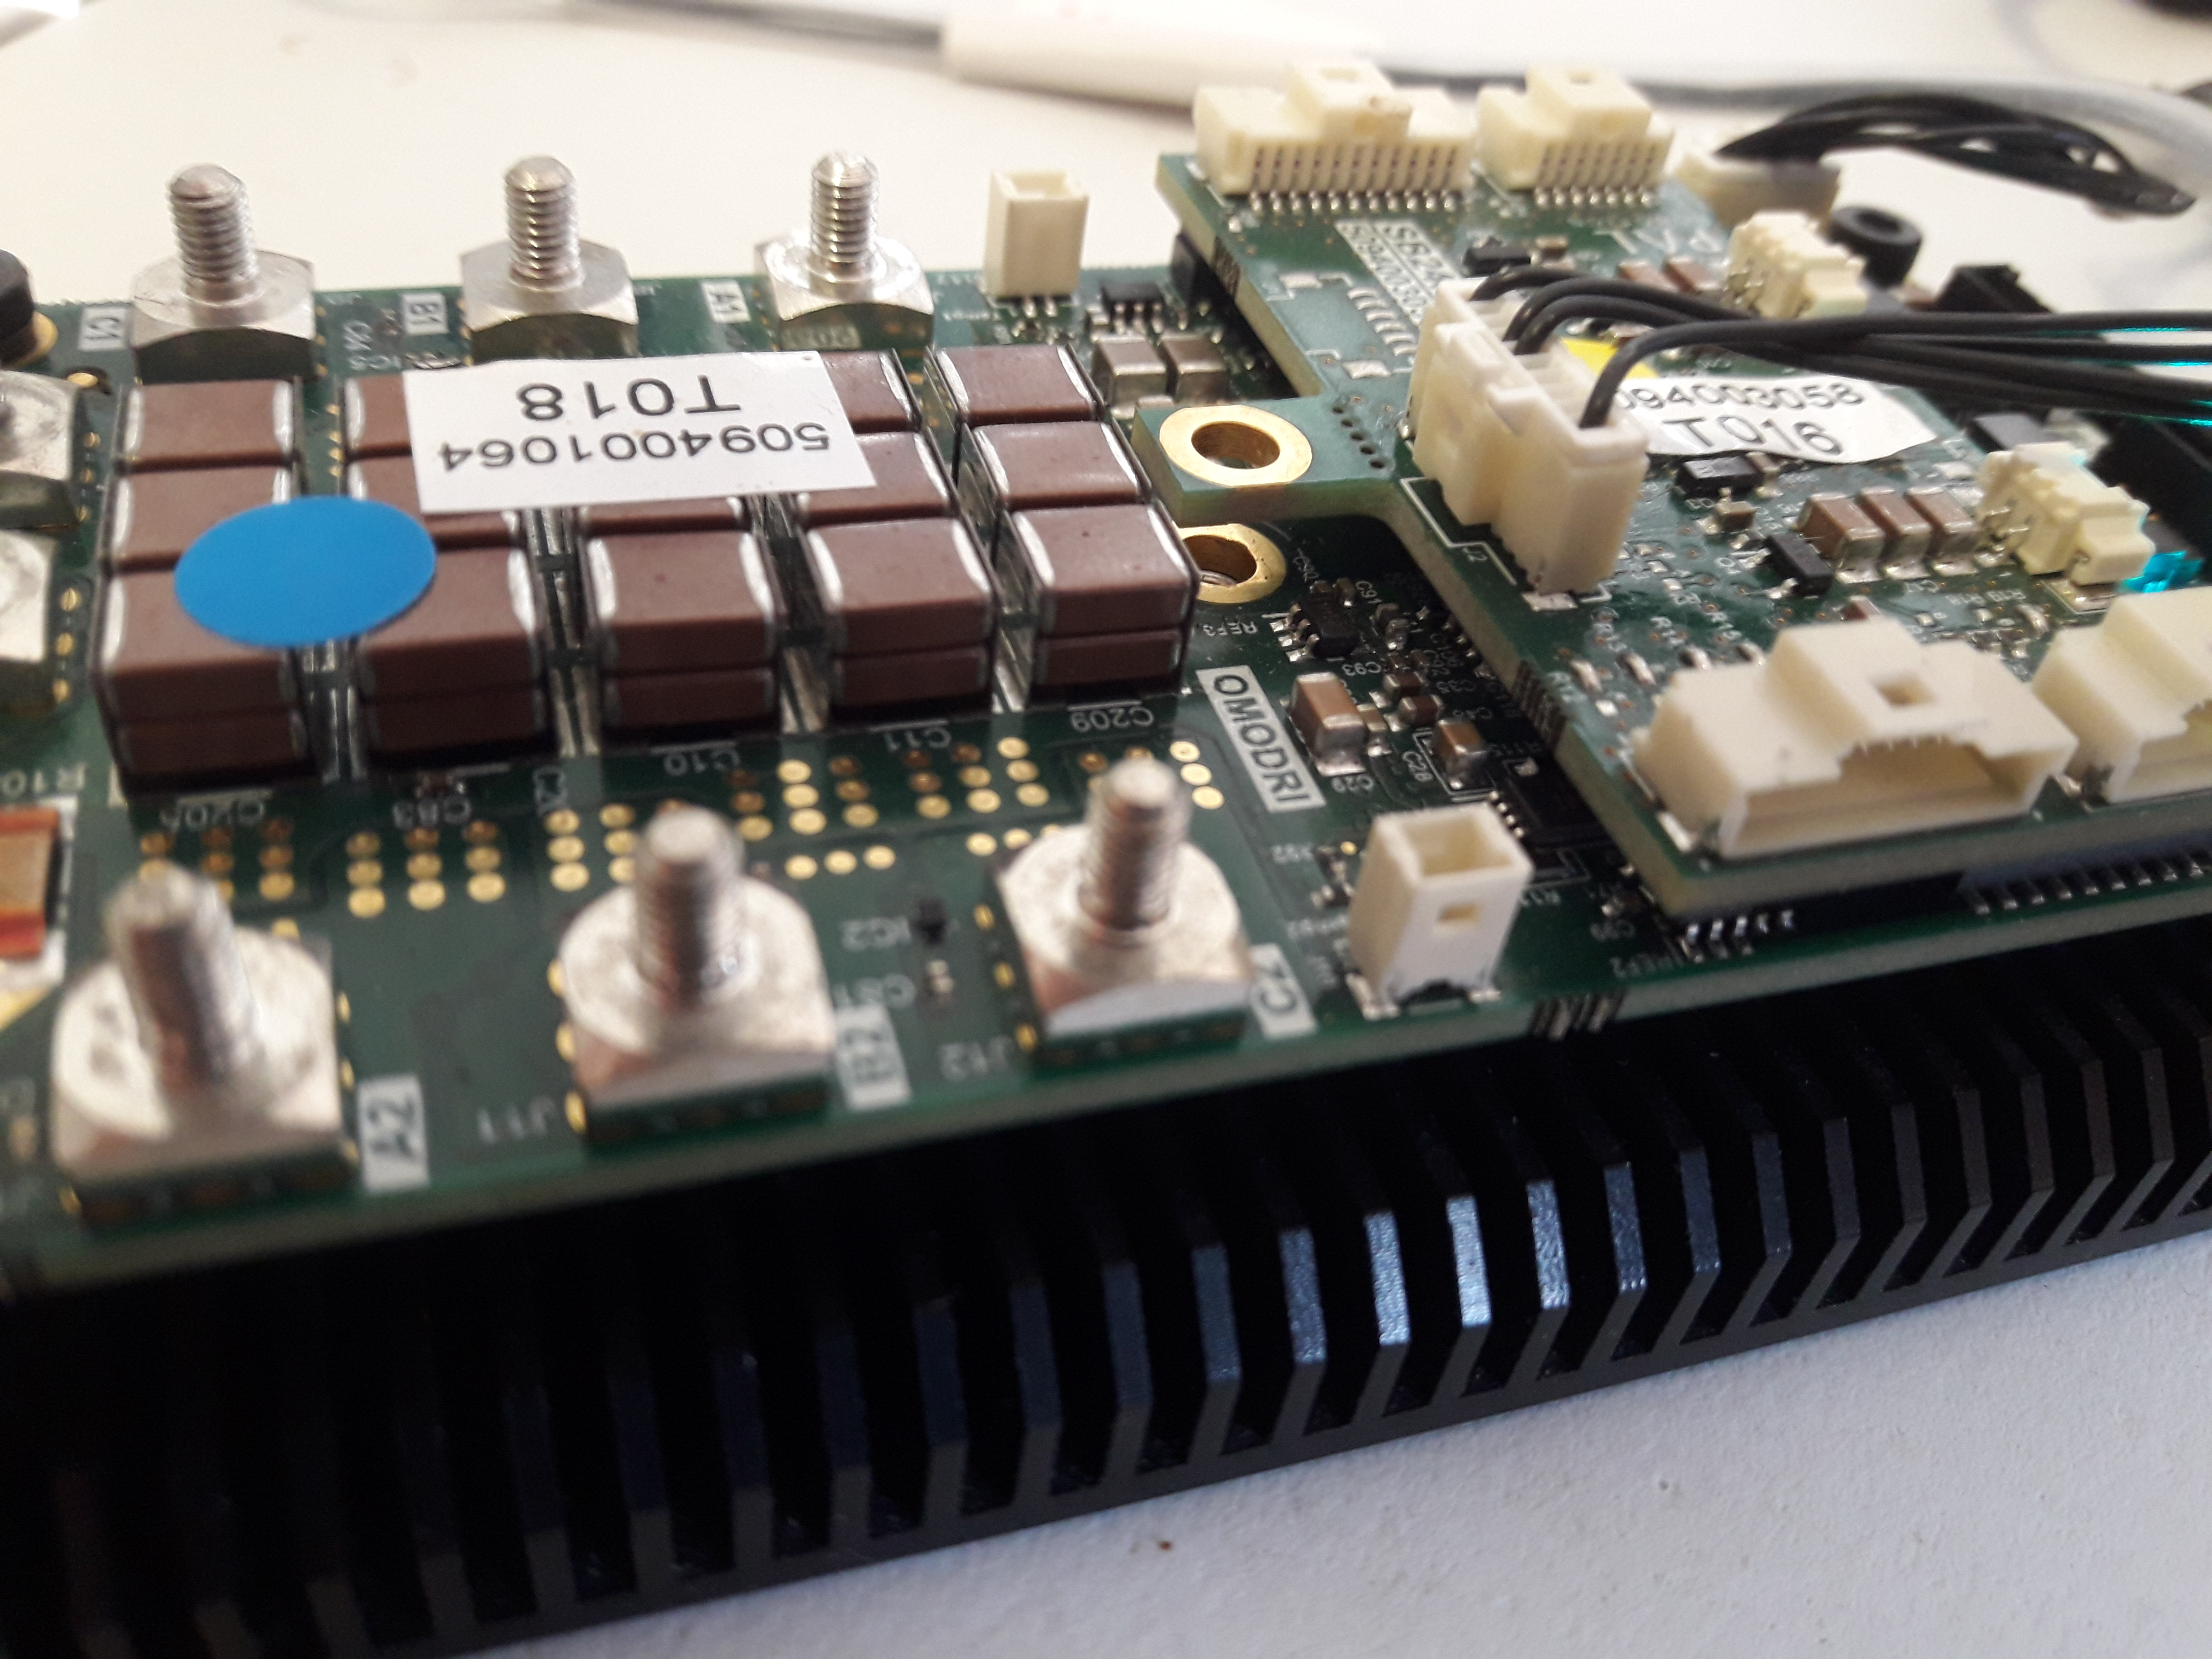
\includegraphics[width=0.3\textwidth]{pal_robotics8.jpg}
            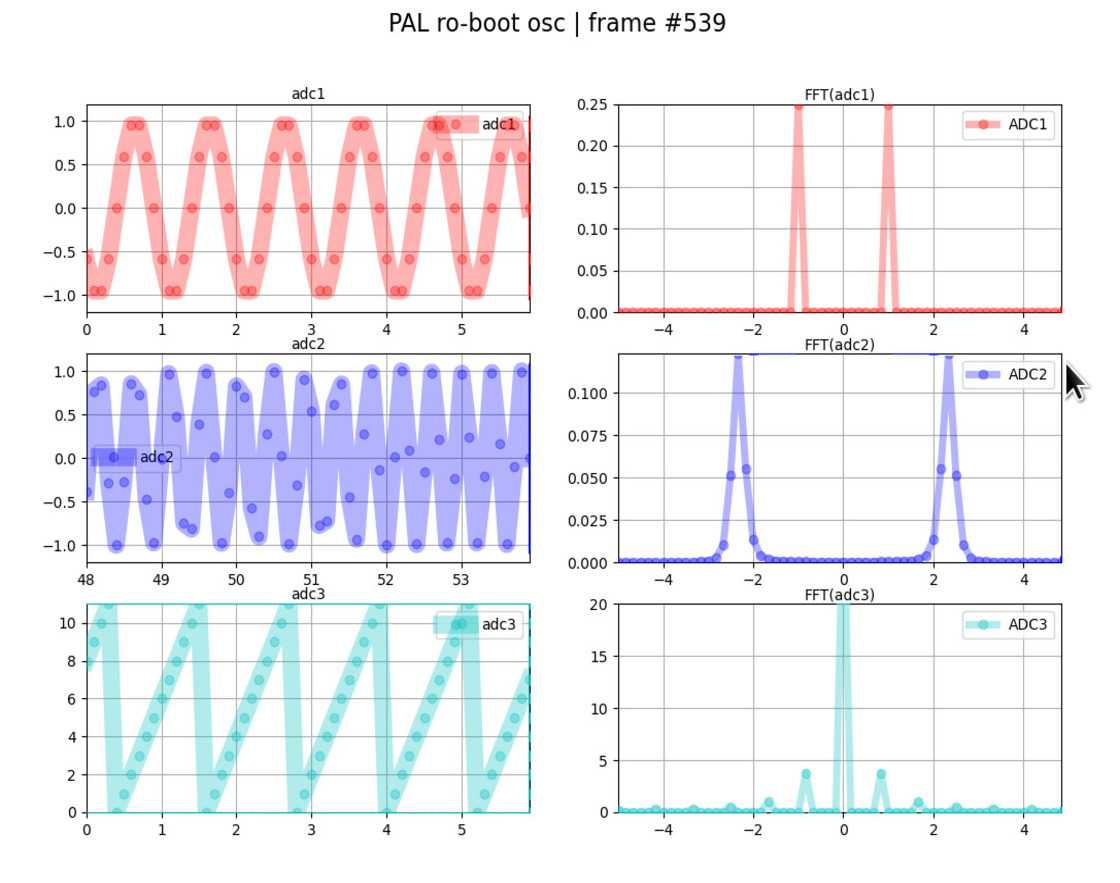
\includegraphics[width=0.3\textwidth]{pal_robotics4.jpg}
            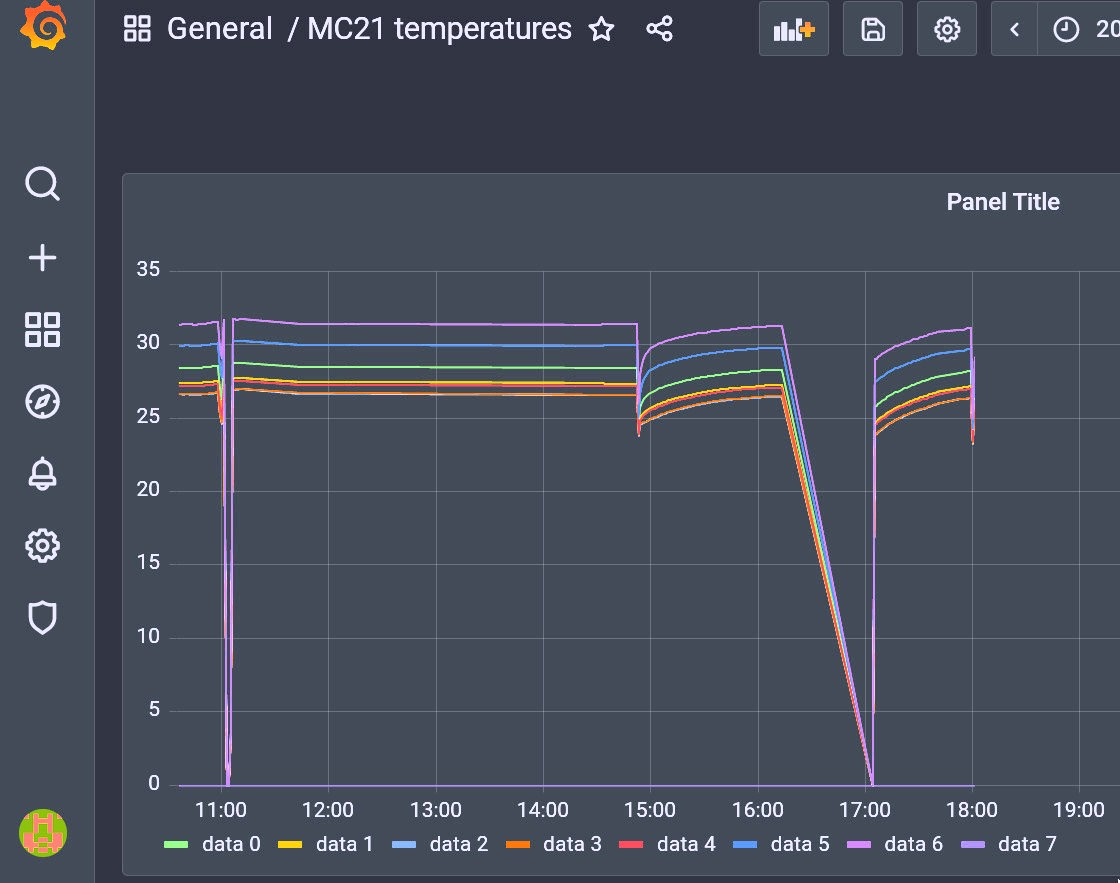
\includegraphics[width=0.3\textwidth]{pal_robotics6.jpg}
         \end{center}
           \caption{Command line to interact with any core with same interface. Realtime matplotlib visualizer. Python -> influxDB <- Grafana persistent data visualizer. }
         \label{fig:novo_space}
      \end{figure}
%---------------------------------------------------
\fi
